\chapter{Neural Networks}
Despite how seemingly popular neural networks have become recently, they aren't actually a novel technique. The first neural networks were described in the early 1940s, and the only reason they weren't put into practice shortly thereafter was the fact that we didn't yet have access to the large amounts of storage and compute that complex neural networks require. Over the last two decades, and particularly with the advent of cloud computing, we now have more and more access to the cheap processing power and memory required to make neural networks a viable option for model building.

As we will come to see in this chapter, neural networks are an extraordinarily flexible class of models used to solve a variety of different problem types. In fact, this flexibility is both what makes them so widely applicable and yet so difficult to use properly. We will explore the applications, underlying theory, and training schemes behind neural networks.

\section{Motivation}
For problems that fall into the category of regression or classification, we've already discussed the utility of basis functions. Sometimes, a problem that is intractable with our raw input data will be readily solvable with basis-transformed data. We often select these basis changes using expert knowledge. For example, if we were working with a data set that related to chemical information, and there were certain equations that a chemist told us to be important for the particular problem we were trying to solve, we might include a variety of the transformations that are present in those equations. If the values of a feature span many orders of magnitude, we might take the logarithm of that feature to make it more manageable for a linear model.

However, imagine now that we have a data set with no accompanying expert information. More often than not, complex problem domains don't come with a useful set of suggested transformations. How do we find useful basis functions in these situations? This is exactly the strength of neural networks - they identify the best basis for a data set!

Neural networks simultaneously solve for our model parameters and the best basis transformations. This makes them exceedingly flexible. Unfortunately, this flexibility is also the weakness of neural nets: while it enables us to solve difficult problems, it also creates a host of other complications. Chief among these complications is the fact that neural networks require a lot of computation to train. This is a result of the effective model space being so large - to explore it all takes time and resources. Furthermore, this flexibility can cause rather severe overfitting if we are not careful.

In summary, neural networks identify good basis transformations for our data, and the strengths and weaknesses of neural networks stem from the same root cause: model flexibility. It will be our goal then to appropriately harness these properties to create useful models.

\subsection{Comparison to Other Methods}
In the previous two chapters, we explored two broad problem types: classification and regression, and it's natural to wonder where neural networks fit in. The answer is that they are applicable to both. The flexibility of neural networks even extends to the types of problems they can be made to handle. Thus, the tasks that we've explored over the last two chapters, such as predicting heights in the regression case or object category in the classification case, can be performed by neural networks.

Given that neural networks are flexible enough to be used as models for either regression or classification tasks, this means that every time you're faced with a problem that falls into one of these categories, you have a choice to make between the methods we've already covered or using a neural network. Before we've explored the specifics of neural networks, how can we discern at a high level when they will be a good choice for a specific problem?

One simple way to think about this is that if we never \textit{needed} to use neural networks, we probably wouldn't. In other words, if a problem can be solved effectively by one of the techniques we've already described for regression or classification (such as linear regression, discriminant functions, etc.), we would prefer to use those. The reason is that neural networks are often more memory and processor intensive than these other techniques, and they are much more complex to train and debug.

The flip side of this is that hard problems are often too complex or too hard to engineer features for to use a simple regression or classification technique. Indeed, even if you eventually think you will need to use a neural network to solve a given problem, it makes sense to try a simple technique first both to get a baseline of performance and because it may just happen to be good enough -- without this check, there is a very real chance that you end up investing time and compute into a neural network that doesn't outperform or generalize better than a linear model. 

What is so special about neural networks that they can solve problems that the other techniques we've explored may not be able to? And why are they so expensive to train? These questions will be explored over the course of the chapter, and a good place to start is with the status of neural networks as universal function approximators.

\subsection{Universal Function Approximation}
The flexibility of neural networks is a well-established phenomenon. In fact, neural networks are what are known as \textit{universal function approximators}. This means that with a large enough network, it is possible to approximate any function. The proof of this is beyond the scope of this textbook, but it provides some context for why flexibility is one of the key attributes of neural networks.

\begin{mlcube}{Neural Networks}
As universal function approximators, neural networks can operate over discrete or continuous outputs. We primarily use neural networks to solve regression or classification problems, which involve training on data sets with example inputs and outputs, making this a \textbf{supervised} technique. Finally, while there exist probabilistic extensions for neural networks, they primarily operate in the \textbf{non-probabilistic} setting.
\begin{center}
    \begin{tabular}{c|c|c}
    \textit{\textbf{Domain}} & \textit{\textbf{Training}} & \textit{\textbf{Probabilistic}} \\
    \hline
    Continuous/Discrete & Supervised & No \\
    \end{tabular}
\end{center}
\end{mlcube}

\section{Feed-Forward Networks}
The feed-forward neural network is the most basic setup for a neural network. Most of the logic behind neural networks can be explained using a feed-forward network, with additional bells and whistles typically added to form more complex networks. We will explore this basic neural network structure first.

\section{Neural Network Basics and Terminology}

\begin{figure}
    \centering
    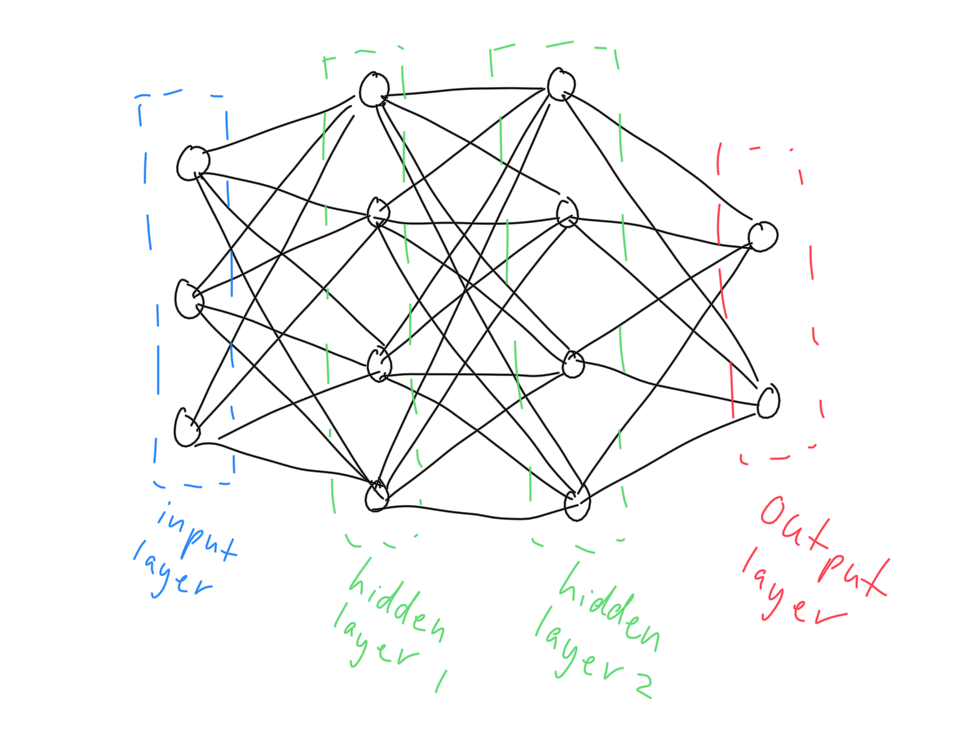
\includegraphics[width=0.5\paperwidth]{../NeuralNetworks/fig/basic-nn.png}
    \caption{Simple Neural Network.}
    \label{fig:basic-nn}
\end{figure}

Looking at Figure \ref{fig:basic-nn}, we see that a feed-forward neural network is a series of connected \textbf{layers} that transform an input data point $\textbf{x}$ into an output data point $\textbf{y}$. Each layer is composed of \textbf{nodes}, the small black circles. Each node in the input layer corresponds to one dimension of a single data point $\textbf{x}$ (meaning the first node is $x_1$, the second node $x_2$, etc.). The same is true of the nodes in the output layer, which represent each dimension of $\textbf{y}$.  For a binary classification problem there is a single output node, representing the predicted probability of the positive class (with $K$ outputs for multi-classification). For a regression problem there may one or more nodes, depending on the dimensions of the output.  The nodes in the  \textbf{hidden} layers correspond to  \textbf{activation functions}.

\begin{figure}
    \centering
    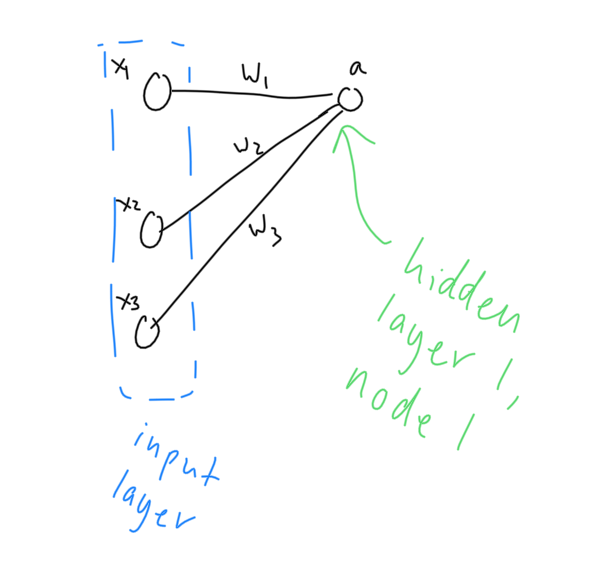
\includegraphics[width=0.5\paperwidth]{../NeuralNetworks/fig/layer-one-node-one.png}
    \caption{Zooming in on the inputs and the first node of the first layer.}
    \label{fig:layer-one-node-one}
\end{figure}

 Let's zoom in on the first node in hidden layer 1, shown in Figure \ref{fig:layer-one-node-one}, to describe what happens at each node as we transform an input. For now we adopt simple notation and don't worry about indexing by later.
Looking at Figure \ref{fig:layer-one-node-one}, notice that every node in the input layer is connected to this first node in hidden layer 1. Each of the lines is a \textbf{connection}, that has a weight $w_{d}$ associated with it. We multiply all the nodes in the input layer by their corresponding weight, and then add them all together to produce the {\em activation} $a$, i..e,  the input at this first node (we've included the bias term in the input vector):
\begin{equation}
	a = x_{1} w_{1} + x_{2} w_{2} + x_{3} w_{3}
\end{equation}
\readernote{Every node in every layer has distinct weights associated with it.}

This gives us the activation for the first node in the first hidden layer. Once we've done this for every node in the first hidden layer, we make a non-linear transform of these activations, and then move on to computing the activations for the second hidden layer (which require the outputs from the first hidden layer, as indicated by the network of connections). We keep pushing values through the network in this manner until we have our complete output layer, at which point we are finished.

We've skipped over some important details in this high-level overview, but with this general information about what a neural network looks like and the terminology associated with it, we can now dig into the details a little deeper.

\subsection{Adaptive Basis Functions}
As we mentioned in the introduction, the strength of neural networks is that we can learn an effective basis for our problem domain at the same time as we train the parameters of our model. In fact, learning this basis becomes just another part of our parameter training. Let's make this notion of learning a basis more concrete.

Thinking back to our chapter on linear regression, we were training a model that made predictions using a functional form that looked like:
\begin{align*}
	y(\textbf{x}, \textbf{w}) = \textbf{w} \boldsymbol{\phi}^{T} = \sum_{d=1}^{D} w_{d} \boldsymbol{\phi}_{d}
\end{align*}
where $\boldsymbol{\phi} = \phi(\textbf{x})$, $\phi$ is the basis transformation function, and $D$ is the dimensionality of the data point.

Typically with this linear regression setup, we are training our model to optimize the parameters $\textbf{w}$. With neural networks this is no different--- we still train to learn those parameters. However, the difference in the neural network setting is that the basis transformation function $\phi$ is no longer fixed. Instead, the transformations are incorporated into the model parameters, and thus learned at the same time.

This leads to a different functional form for neural networks. A neural network with $M$ nodes in its first hidden layer  performs $M$ linear combinations of an input data point $\textbf{x}$:
\begin{equation} \label{basic-nn-form}
	a^{(1)}_{j} = \sum_{d=1}^{D} w_{jd}^{(1)} x_{d} + w_{j0}^{(1)} \quad \forall j \in 1..M
      \end{equation}

      Here, we use $a^{(1)}$ to denote the activation of a unit in layer 1 and notation $w^{(1)}$  denotes the weights used to determine the activations in layer 1. We also make the bias explicit.
      We will still use the bias trick in general, but we've left it out here to
      explicitly illustrate the bias term
      $w_{j0}^{(1)}$.
      %
      Other than this,  equation \ref{basic-nn-form} describes what we've already seen in Figure \ref{fig:layer-one-node-one}. The only difference is that we index each node in the hidden layer (along with its weights) by $j$.
      %There are $M$ nodes in this first hidden layer, corresponding to the $M$ linear combinations of the input data point $\textbf{x}$.
      %The notation $w^{(1)}$ indicates that these weights are part of the first hidden layer of our network.

      %Notice also that we haven't applied the `bias trick' of appending a $1$ to our data point $\textbf{x}$.
      
      The $M$ different values $a^{(1)}_{j}$ are the  activations. We transform these activations with a non-linear activation function $h(\cdot)$ to give:
      %
\begin{equation} \label{basic-nn-z-outputs}
	z^{(1)}_{j} = h(a_{j})
      \end{equation}
      
\readernote{Note that we didn't mention activation functions in the previous section only for the sake of simplicity. These non-linearities are crucial to the performance of neural networks because they allow for modeling of outcomes that vary non-linearly with their input variables.}

These values $z^{(1)}_{j}$ correspond to the outputs of the hidden units, each of which is associated with an activation function. Superscript $^{(1)}$ indicates they are the outputs of units in layer 1.
A typical activation function is the  sigmoid function, but  other common choices are the {\em tanh function} and {\em  rectified linear unit (ReLU)}.

These output values $z^{(1)}_{j}$, for units $j\in \{1,\ldots,M\}$ in layer 1,
form the inputs to the next layer. The activation of unit $j'$ in layer 2 depends on the outputs from layer 1 and the weights $w^{(2)}_{j'0},w^{(2)}_{j'1},\ldots,w^{(2)}_{j'M}$ that define the linear sum at the input of unit $j'$:
%
\begin{equation} \label{basic-nn-form-next-layer}
	a^{(2)}_{j'} = \sum_{j=1}^{M} w_{j'm}^{(2)} z^{(1)}_{j} + w_{j'0}^{(2)}
      \end{equation}
      
      We can connect many layers together in this way. They need not all have the same number of nodes but we will adopt $M$ for the number of nodes in each layer for convenience of exposition. Eventually, we will reach the output layer, and each output is denoted $y_{k}$, for $k\in \{1,\dots,K\}$.
      %
      The final activation function may be the sigmoid function, softmax function, or  just linear (and thus no transform).
      
We can now examine a more complete diagram of a feed-forward neural network, shown in Figure \ref{fig:feed-foward-nn}. It may be helpful to reread the previous paragraphs and use the diagram to visualize how a neural network transforms its inputs. This is a single hidden layer, or two-layer, network. Here, we use $z$ to denote the output values of the units in the hidden layer.

\begin{figure}
    \centering
    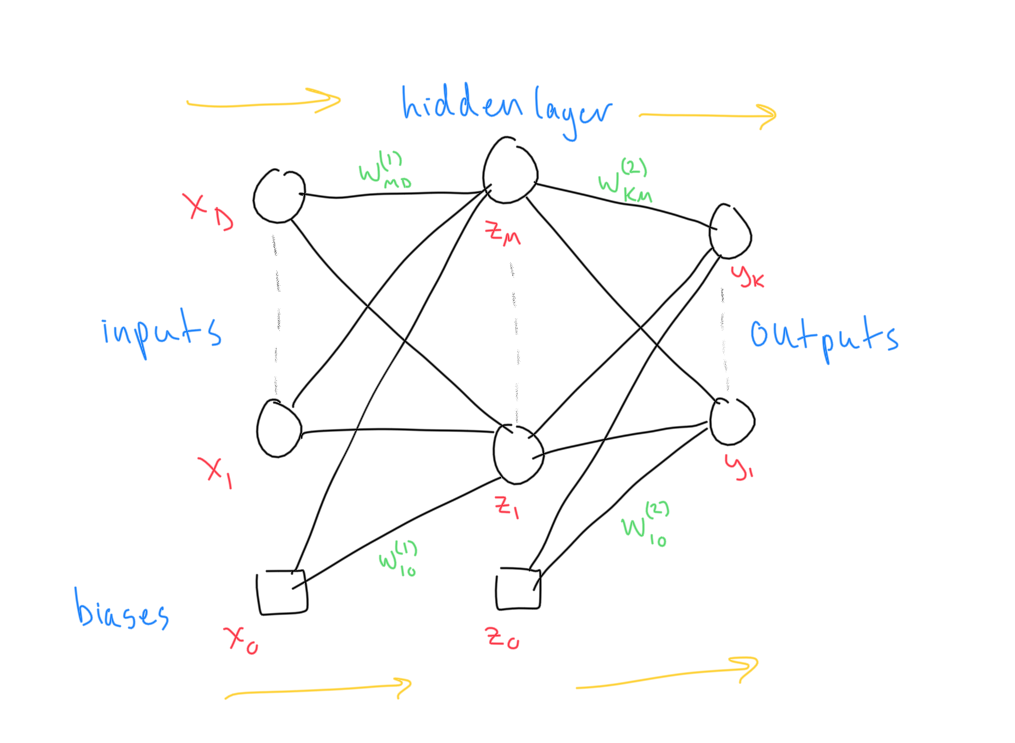
\includegraphics[width=0.5\paperwidth]{../NeuralNetworks/fig/feed-forward-nn.png}
    \caption{Feed-Forward Neural Network.}
    \label{fig:feed-foward-nn}
\end{figure}

\readernote{Different resources choose to count the number of layers in a neural net in different ways. We've elected to count each layer of non-input nodes, thus the two-layer network in Figure \ref{fig:feed-foward-nn}. However, some resources will choose to count every layer of nodes (three in this case) and still others count only the number of hidden layers (making this a one layer network).}

Combining Figure \ref{fig:feed-foward-nn} and our preceeding functional description, we can describe the operation performed by a two-layer neural network using a single functional transformation (with $m$ to index a unit in the hidden layer):
%
\begin{equation} \label{full-nn-equation}
	y_{k}(\textbf{x}, \textbf{w}) = \sigma\bigg(\sum_{m=1}^{M}w_{km}^{(2)} h\bigg(\sum_{d=1}^{D}w_{md}^{(1)}x_{d} + w_{m0}^{(1)}\bigg) + w_{k0}^{(2)}\bigg)
\end{equation}
where we've elected to make the final activation function the sigmoid function $\sigma(\cdot)$, as is suitable for binary classification.  We use $h$ to denote the non-linear activation function for a hidden unit.
%
Written like this, a neural network is simply a non-linear function that transforms an input $\textbf{x}$ into an output $\textbf{y}$ that is controlled by our set of parameters $\textbf{w}$.

Furthermore, we see now why this  basic variety of neural networks is a \textit{feed-forward neural network}. We're  simply feeding our input \textbf{x} forward through the network from the first layer to the last layer. Assuming we have a fully trained network, we can make predictions on new input data points by propagating them through the network to generate output predictions (``the forward pass'').

We can also simplify this equation by utilizing the bias trick and appending an $x_{0}=1$ value to each of our data points such that:
\begin{equation*}
	y_{k}(\textbf{x}, \textbf{w}) = \sigma\bigg(\sum_{m=1}^{M}w_{km}^{(2)} h\bigg(\sum_{d=1}^{D}w_{md}^{(1)}x_{d}\bigg)\bigg)
\end{equation*}

Finally, it's worth considering that while a neural network is a series of linear combinations, it is special because of the differentiable non-linearities applied at each of the hidden layers. Without these non-linearities, the successive application of different network weights would be equivalent to a single large linear combination.

%Now that we understand the basic structure of a neural network, the important question of how to train our network remains. This is the topic we turn to next.

\section{Network Training}
Now that we understand the structure of a basic feed-forward neural network and how they can be used to make predictions, we turn our attention to the training process.

\subsection{Objective Function}

To train our network, it's first necessary to establish an objective function. Remember that neural networks can be used to solve both regression and classification problems, which means that our choice of objective will depend on the type of problem and the properties we desire.

For the case of {\em linear regression}, a common objective function is the {\em least squares loss}:
%
\begin{equation} \label{least-squares-loss-function}
	\mathcal{L}(\textbf{w}) = \frac{1}{2} \sum_{n=1}^{N} \bigg(y(\textbf{x}_{n}, \textbf{w}) - y_n\bigg)^{2},
      \end{equation}
      %
      where $y_n$ is the target value on example $n$. Sometimes we will have a regression problem with multiple outputs, in which case the loss would also take the sum over these different target values.
      
      For a {\em binary classification} problem, which we model through a single, sigmoid output activation unit,
     then  negated log-likelihood (or cross-entropy) is the typical  loss function:
      %
\begin{equation} \label{cross-entropy-loss-function}
	\mathcal{L}(\textbf{w}) = - \sum_{n=1}^{N} \bigg(y_{n}\ln{\hat{y}_{n}} + (1 - y_{n})(\ln{(1 - \hat{y}_{n})}\bigg)
      \end{equation}
      
      For a {\em multiclass classification problem}, produced by a softmax function in the output activation layer, we
      would use the negated log likelihood (cross entropy) loss:
\begin{equation} \label{multiclass-cross-entropy-loss-function}
	\mathcal{L}(\textbf{w}) = - \sum_{n=1}^{N} \sum_{k=1}^{K} y_{kn} \ln{\bigg(\frac{\text{exp}(a_{k}(\textbf{x}, \textbf{w}))}{\sum_{j=1}^{K}\text{exp}(a_{j}(\textbf{x}, \textbf{w}))}\bigg)}
\end{equation}

\readernote{Loss function and  objective function all refer to the same concept: the function we optimize to train our model.}

\subsection{Optimizing Parameters}

We want to find weight parameters \textbf{w} to minimize the objective function. The highly non-linear nature of neural networks means that this objective function will be non-convex with respect to our weight parameters. But still, we make use of stochastic gradient descent for optimization (refer to the previous chapter for a refresher).

In order to use gradient descent, we first need to figure out how to compute the gradient of our objective function with respect to our weights. That is the topic of the next section.

\subsection{Backpropagation}

Considering how our feed-forward neural network works, by propagating activations through our network to produce a final output, it's not immediately clear how we can compute gradients for the weights that lie in the middle of our networ. There is an elegant solution to this, which comes from ``sending errors backwards'' through our network, in a process known as \textit{backpropagation}.

\begin{definition}{Backpropagation}{backpropagation}
  
Backpropagation is the procedure by which we pass errors backwards through a feed-forward neural network in order to compute gradients for the weight parameters of the network.
\end{definition}

Backpropagation refers specifically to the portion of neural network training during which we compute the derivative of the objective function with respect to the weight parameters. This is done by propagating errors backwards through the network, hence the name.

\readernote{Note that we still need to update the value of the weight parameters after computing their derivatives. This is typically done using gradient descent or some variant of it.}

We now explore the details of backpropagation in greater depth.

\subsection{Computing Derivatives Using Backpropagation}

Recall that the activation $a_{j}^{(\ell)}$ for a  node $j$ in layer $\ell$ of a neural network can be described by the equation:
\begin{equation} \label{activations-reminder}
	a_{j}^{(\ell)} = \sum_{m=1}^{M} w^{(\ell)}_{jm} z^{(\ell-1)}_{m},
      \end{equation}
      % hull
where there are $M$ incoming nodes, each with corresponding output values $z^{(\ell-1)}_{1}, ..., z^{(\ell-1)}_{M}$, and with the weights in layer $\ell$ corresponding to node $j$ denoted by $w^{(\ell)}_{j1}, ..., w^{(\ell)}_{jM}$.
This activation is transformed by an activation function $h(\cdot)$  to give unit output $z^{(\ell)}_{j}$:
\begin{equation} \label{transformed-activations-reminder}
	z^{(\ell)}_{j} = h(a^{(\ell)}_{j}).
\end{equation}

Computing these values as we flow through the network constitutes the {\em forward pass } through our network.

We now wish to begin the process of computing derivatives of the objective function with respect to our weights. For the sake of simplicity, we'll assume that the current setting of our parameters $\textbf{w}$ generates a loss of $L$ for a single data point, as though we were performing stochastic gradient descent.

Let's consider how we could compute the derivative of $L$ with respect to an individual weight in our network, $w^{(\ell)}_{jm}$ (the $m$th weight for activation $j$ in layer $\ell$):
%
\begin{equation} \label{deriv-E-wrt-wjm}
	\frac{\partial L}{\partial w^{(\ell)}_{jm}}.
\end{equation}

We first need to figure out what the dependence of $L$ is on this weight. This weight contributes to the final result only via its contribution to the activation $a^{(\ell)}_{j}$. This allows us to use the chain rule to simplify Equation \ref{deriv-E-wrt-wjm} as:
%
\begin{equation} \label{chain-rule-deriv-E-wrt-wjm}
	\frac{\partial L}{\partial w^{(\ell)}_{jm}} = \frac{\partial L}{\partial a^{(\ell)}_{j}} \cdot \frac{\partial a^{(\ell)}_{j}}{\partial w^{(\ell)}_{jm}}.
      \end{equation}

      The first part of this is the, typically non-linear, dependence of loss on activation. The second part is the linear dependence of activation on weight.
      %
Using Equation \ref{activations-reminder}, we have that:
\begin{equation*}
	\frac{\partial a^{(\ell)}_{j}}{\partial w^{(\ell)}_{jm}} = z^{(\ell-1)}_{m},
\end{equation*}

and just the value of the input from the previous layer. We now introduce the following notation for the first term,
%
\begin{equation} \label{delta-expression}
	\delta^{(\ell)}_{j} = \frac{\partial L}{\partial a^{(\ell)}_{j}},
\end{equation}
where $\delta^{(\ell)}_{j}$ values are referred to as \textit{errors}. We rewrite Equation \ref{chain-rule-deriv-E-wrt-wjm} as:
%
\begin{equation} \label{simplified-chain-rule-deriv-E-wrt-wjm}
	\frac{\partial L}{\partial w^{(\ell)}_{jm}} = \delta^{(\ell)}_{j} z^{(\ell-1)}_{m}.
\end{equation}

The implications of Equation \ref{simplified-chain-rule-deriv-E-wrt-wjm} are significant for understanding backpropagation.  The derivative of the loss with respect to an arbitrary weight in the network
can be calculated as the product of the error $\delta^{(\ell)}_j$ at the ``output end of that weight'' and the value $z^{(\ell-1)}_m$ at the ``input end of the weight.''  We visualize this property in Figure \ref{fig:backprop-gradient} (dropping the layer subscripting).
%
\begin{figure}
    \centering
    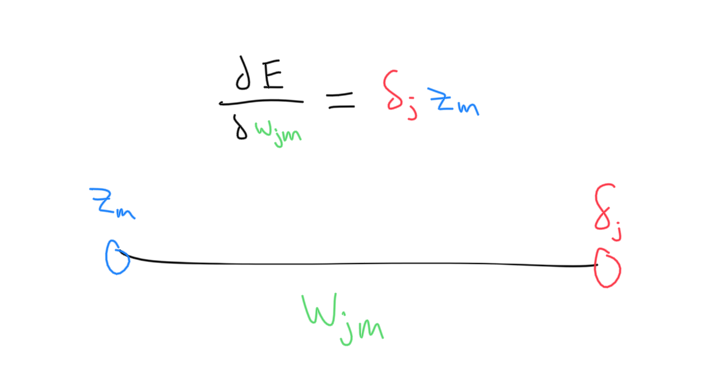
\includegraphics[width=0.5\paperwidth]{../NeuralNetworks/fig/backprop-gradient.png}
    \caption{Gradient of the loss function in a neural network with respect to a weight. It depends on the input value $z_m$ and the ``error'' corresponding to the activation value at the output end of the weight.}
    \label{fig:backprop-gradient}
\end{figure}

To compute the derivatives, it suffices to compute the values of $\delta_{j}$ for each node, also saving the output values  $z_{m}$ during the forward pass through the network (to be multiplied by the values of $\delta_{j}$ to get partials).

\readernote{We will only have ``errors values'' $\delta_{j}$ for the hidden and output units of our network. This is logical because there is no notion of applying an error to our input data, which we have no control over.}

We now consider how to compute these error values.  For a unit in the output layer, indexing it here by $k$,  and assuming the output activation function is linear and adopting least squares loss (i.e., regression), we have  for the dependence of loss on the activation of this unit,
%
\begin{equation*}
  \delta^{(\ell)}_{k} = \frac{\partial L}{\partial a^{(\ell)}_k} =
 \frac{\partial L}{\partial \hat{y}_k} =
  \frac{\mathrm{d} \big( \frac{1}{2}(\hat{y}_k- y_k)^2 \big)}{\mathrm{d} \hat{y}_{k}} = \hat{y}_{k} - y_{k}.
\end{equation*}

Here, we use shorthand $a^{(\ell)}_k=\hat{y}_k$, providing the $k$th dimension of the  prediction  of the  model. Although a regression problem, we're imagining here that there are multiple regression targets (say, the height, weight and blood pressure of an individual). Here, $y_k$ is the true target value for this data point. Note that this is for OLS. The expression would be different for a classification problem and negated log likelihood as the loss.

\if 0
The error $\delta_k^{(\ell)}$ on a unit in the output layer, for this case of OLS, is the difference between the output of the network and the target value. We've seen this term, the difference between the expected and actual results, arise in the gradient of our error expressions for both linear regression and classification.
\fi

To compute the error $\delta^{(\ell)}_{j}$ for a hidden unit $j$ in a layer $\ell$, we again make use of the chain rule, and write:
%
\begin{equation} \label{backprop-for-deltas}
	\delta^{(\ell)}_{j} = \frac{\partial L}{\partial a^{(\ell)}_{j}} = \sum_{m=1}^{M} \frac{\partial L}{\partial a^{(\ell+1)}_{m}} \frac{\partial a^{(\ell+1)}_{m}}{\partial a_{j}^{(\ell)}}, 
\end{equation}
where the summation runs over all of the $M$ nodes to which the node $j$ in layer $\ell$ sends connections, as seen in Figure \ref{fig:sum-over-nodes}. This expression recognizes that the activation value of this unit contributes only via its contribution to the activation value of each unit to which it is connected in the next layer. The first term in
one of the  products in the summation is the, typically non-linear, dependence between loss and activation value of a unit in the next layer. The second term in one of the products captures the relationship between this activation and the subsequent activation.
%
%
\begin{figure}
    \centering
    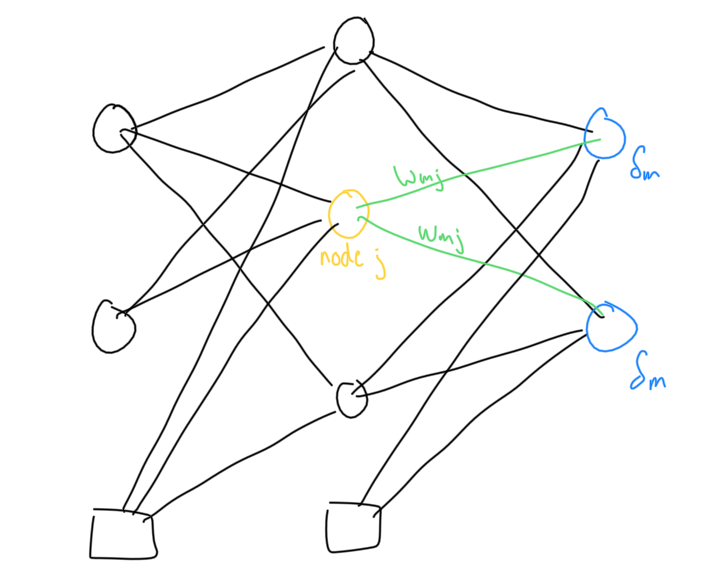
\includegraphics[width=0.5\paperwidth]{../NeuralNetworks/fig/sum-over-nodes.png}
    \caption{Summation over the nodes (blue) in layer $\ell+1$ to which node $j$ in layer $\ell$ (gold) sends connections (green). Note: read this as $m$ and $m'$.}
    \label{fig:sum-over-nodes}
\end{figure}

Now, we can simplify by noticing that:
%
\begin{align}
  \frac{\partial L}{\partial a_m^{(\ell+1)}}&=\delta^{(\ell+1)}_m \quad\quad\mbox{\{by definition\}}\\
  \frac{\partial a_m^{(\ell+1)}}{\partial a_j^{(\ell)}}&=\frac{\mathrm{d}h(a_j^{(\ell)})}{\mathrm{d}a_j^{(\ell)}}\cdot w^{(\ell+1)}_{mj}=h'(a_j^{(\ell)})\cdot w_{mj}^{(\ell+1)}. \quad\quad\mbox{\{chain rule\}}
\end{align}

Substituting, and pulling forward the derivative of the activation function, we can rewrite the expression for the error on a hidden unit $j$ in layer $\ell$ as:
%
\begin{equation} \label{backprop-formula}
	\delta^{(\ell)}_{j} = h'(a^{(\ell)}_{j}) \sum_{m=1}^{M} w^{(\ell+1)}_{mj} \delta^{(\ell+1)}_{m}.
      \end{equation}

      This is very useful, and is the key insight in backpropagation.  It means that the value of the errors  can be computed by ``passing back'' (backpropagating) the errors for  nodes farther up in the network! 
%
Since we know the values of $\delta$ for the final layer of output node, we can recursively apply Equation \ref{backprop-formula} to compute the values of $\delta$ for all the nodes in the network.

Remember that all of these calculations were done for a single input data point that generated the loss $L$. If we were using SGD with  mini-batches, then we would perform  same calculation for each data point in mini-batch $B$, and average the gradients as follows:
%
\begin{equation} \label{batch-errors-backprop}
	\frac{\partial L}{\partial w^{(\ell)}_{jm}} = \frac{1}{|B|}\sum_{n\in B} \frac{\partial L_{n}}{\partial w^{(\ell)}_{jm}},
      \end{equation}
      %
      where $L_n$ is the loss on example $n$.
     
Fundamentally, backpropagation is the phrase we use to describe the use of the chain rule on the function implied by the architecture of the neural network. To solidify our understanding of the backpropagation algorithm, it can be useful to try a concrete example.
%
\begin{example}{Backpropagation Example}{backprop-example}
  Imagine the case of a simple two layer neural network as in Figure \ref{fig:feed-foward-nn}, with $K$ outputs (we denote them $\hat{y}_1$ through $\hat{y}_K$ for a given data point). We imagine this is a regression problem, but one
  with multiple dimensions to the output, and assume OLS. For a given data point, the loss is computed as:
   %
	\begin{align*}
		L = \sum_{k=1}^{K} \frac{1}{2}(\hat{y}_{k} - y_{k})^{2},
	\end{align*}
        %
        where we write $y_k$ for the $k$th dimension of the target value.
%
        For a unit in the hidden layer, with activation value $a$, we make use of the sigmoid activation, with 
        %
	\begin{align*}
z=		\sigma(a) = \frac{1}{1 + \exp{(-a)}},
	\end{align*}
	whose derivative is given by:
	\begin{align*}
		\frac{\partial \sigma(a)}{\partial a} = \sigma(a)(1 - \sigma(a)).
	\end{align*}
        
	For an input data point $\textbf{x}$, we forward propagate through the network to get the activations of the hidden layer, and for each $m$ in this layer we have:
	\begin{align*}
		a_{m}^{(1)} = \sum_{d=0}^{D} w^{(1)}_{md} x_{d},
	\end{align*}
    given weights $w^{(1)}_{m0},\ldots, w^{(1)}_{mD}$,   and  with output value from unit $m$ as, 
%
	\begin{align*}
		z^{(1)}_{m} = \sigma{(a^{(1)}_{m})}.
	\end{align*}
        
	We propagate these output values  forward to get the outputs, and for each output unit $k$, we have:
	\begin{align*}
		\hat{y}_{k} = \sum_{m=0}^{M} w_{km}^{(2)} z^{(1)}_{m},
	\end{align*}
        %
where $w^{(2)}_{k0},\ldots,w^{(2)}_{kM}$ are the weights for unit $k$.
        
	Now that we've propagated forward, we propagate our errors backwards! We start by computing the errors for the output layer as follows:
	\begin{align*}
		\delta^{(2)}_{k} =  \frac{\partial L}{\partial \hat{y}_k}=\hat{y}_{k} - y_{k}.
	\end{align*}

	We then backpropagate these errors back to each hidden unit $m$ in layer 1 as follows:
	\begin{align*}
          \delta^{(1)}_{m} = \frac{\partial L}{\partial a_m^{(1)}} & =
                                                                     h'(a_m^{(1)})\sum_{k=1}^Kw^{(2)}_{km}\delta^{(2)}_k\\
                                                                   &=\sigma(a^{(1)}_m)(1-\sigma(a^{(1)}_m))\sum_{k=1}^Kw^{(2)}_{km}(\hat{y}_k-y_k)\\
                                                                   &=z_m^{(1)}(1-z_m^{(1)}) \sum_{k=1}^Kw^{(2)}_{km}(\hat{y}_k-y_k).
                                                                     \end{align*}

	And now that we have our errors for the hidden and output layers, we can compute the derivative of the loss with respect to our weights as follows, for the $d$th weight on the $m$th unit in layer 1, and the $m$th weight on the $k$th unit in layer 2: 
	\begin{align*}
		\frac{\partial L}{\partial w_{md}^{(1)}} = \delta^{(1)}_{m} x_{d}, \quad \frac{\partial L}{\partial w^{(2)}_{km}} = \delta^{(2)}_{k} z^{(1)}_{m}.
	\end{align*}
        
	We then use these derivatives along with an optimization technique such as stochastic gradient descent to improve the model weights.
\end{example}

\section{Choosing a Network Structure}
Now that we know the general form of a neural network and how the training process works, we must step back and consider the question of how we actually arrive at an optimal network structure. We'll begin with an idea we've already seen before: cross validation.

\subsection{Cross Validation for Neural Networks}
We've previously discussed cross validation in the chapter on linear regression. We used it then to compare the performance of different models, attempting to identify the best model while also avoiding overfitting. We can use a similar process to identify a reasonable network structure.

First of all, the input and output parameters of a neural network are generally decided for us: the dimensionality of our input data dictates the number of input units and the dimensionality of the required output dictates the number of output units. For example, if we have an 8-by-8 pixel image and need to predict whether it is a `0' or a `1', our input dimensions are fixed at 64 and our output dimensions are fixed at 2. Depending on whether you wish to perform some sort of pre or post-processing on the inputs/outputs of your network, this might not actually be the case, but in general when choosing a network structure we don't consider the first or last layer of nodes as being a relevant knob that we can tune.

That leaves us to choose the structure of the hidden layers in our network. Unsurprisingly, the more hidden layers we have and the more nodes we have in each of those layers, the more variation we will produce in our results and the closer we will come to overfitting. Very generally, the more free parameters the model can train, the more likely it is to overfit in the same way a linear model with a higher-dimensional basis would. 

Thus, we can use cross validation in the same way we've done before: train our model with differing numbers of internal units and structures (as in Figure \ref{fig:internal-node-differences}) and then select the model that performs best on the validation set.

\begin{figure}
    \centering
    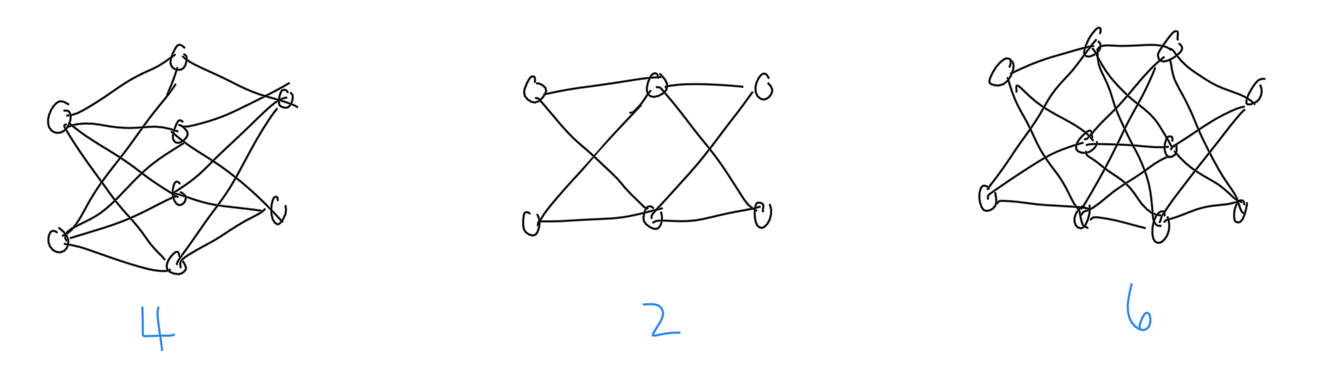
\includegraphics[width=0.5\paperwidth]{../NeuralNetworks/fig/internal-node-differences.png}
    \caption{Networks with different structures and numbers of internal nodes.}
    \label{fig:internal-node-differences}
\end{figure}

\readernote{There are other considerations at play beyond performance when choosing a network structure. For example, the more internal units you have in your network, the more storage and compute time you will need to train them. If either training time or response time after training a model is critical, you may need to consider consolidating your network at the expense of some performace.}

\subsection{Preventing Overfitting}
Besides keeping your neural network small, there are other means of preventing it from overfitting.

\subsubsection{Regularization}
You can also apply regularization to the weights in your network to help prevent overfitting. For example, we could introduce a simple quadratic regularizer of the form $\frac{\lambda}{2} \textbf{w}^{T}\textbf{w}$ to our objective function. There are other considerations to be made here, for example we would like our regularizer to be invariant to scaling, meaning that multiplying our input data by a constant would produce a proportionally equivalent network after training. The quadratic regularizer is not invariant to scaling, but the basic concept of avoiding extreme weights is the same nonetheless.

\subsubsection{Data Augmentation}
We can use transformations to augment our data sets, which helps prevent overfitting. This technique is not specific to neural networks, but often the types of unstructured data for which we use neural networks can benefit greatly from it.
\begin{definition}{Data Augmentation}{data-augmentation}
Data augmentation refers to the practice of increasing the size and diversity of your training data by applying transformations to the initial data set.
\end{definition}
For example, if we are working with image data, we might choose to rotate or reflect the image, depending on the type of network we are trying to build and whether or not this would preserve the integrity of the image. We might also change something like the brightness or density of the image data. In this way, we can produce more and more varied training points, thus reducing the likelihood of overfitting.

\section{Specialized Forms of Neural Networks}
Simple neural networks are useful for a general set of tasks, and as universal function approximators, they \textit{could} be useful for any task. However, there are certain data types and use cases for which we've developed more specialized forms of neural networks that perform even better in their respective domains. We will take a high level view of these different flavors of neural networks.

\subsection{Convolutional Neural Networks (CNNs)}
Convolutional neural networks (abbreviated CNNs) are most often used for image data, but their underlying principles apply in other domains as well.

To understand why a CNN is useful, consider this specific problem: you are trying to determine whether or not there is a dog in an image. There are two general difficulties we have to deal with in solving this problem. First, while dogs have a lot of similar features (ears, tails, paws, etc.), we need some means of breaking an image down into smaller pieces that we can identify as being ears or tails or paws. Second, what happens if we train on images of dogs that are all in the center of the photo, and then we try to test our network on an image where the dog is in the upper left hand corner? It's going to fail miserably.

CNNs overcome these problems by extracting smaller local features from images via what's known as a \textit{sliding window}. You can imagine this sliding window as a matrix kernel that moves over every subsection of an image, producing a summary of those subsections that feed into the next layer in our network. We do this over the entire image, and with several different sliding windows. Without going into too many details, this solves the two general problems we had above: our small sliding window can summarize a feature of interest (such as a dog ear) and it is also location invariant, meaning that we can identify that dog ear anywhere in an image.

\begin{figure}
    \centering
    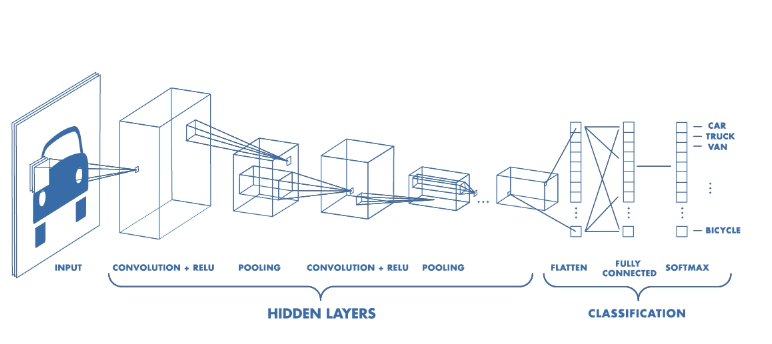
\includegraphics[width=0.5\paperwidth]{../NeuralNetworks/fig/CNN-structure.png}
    \caption{Excellent diagram of the structure of a CNN. source: https://www.mathworks.com/videos/introduction-to-deep-learning-what-are-convolutional-neural-networks--1489512765771.html}
    \label{fig:CNN-structre}
\end{figure}

\subsection{Recurrent Neural Networks (RNNs)}
As with CNNs, recurrent neural networks (abbreviated RNNs) are used to more efficiently solve a specific problem type. To motivate the structure of an RNN, we will turn again to a specific example.

Imagine we were building a tool with the goal of predicting what word comes next in a newspaper article. Obviously, the words that came before the word that we are currently trying to predict are crucial to predicting the next word. Imagine we propagate the preceding ten words through our network to predict which word we think will come next. It would also be useful if we could send some of the information at each layer backwards through the network to help with the next prediction - since we know the sequence of words matters. In this sense, our network is `stateful' because it's remembering what came before. We don't have this ability with a feed-forward network, which by design only propagates information forward through the network. RNNs add backward passing of activations into their network structure to improve predictions on data where there is some temporal dependence on what came previously.

\begin{figure}
    \centering
    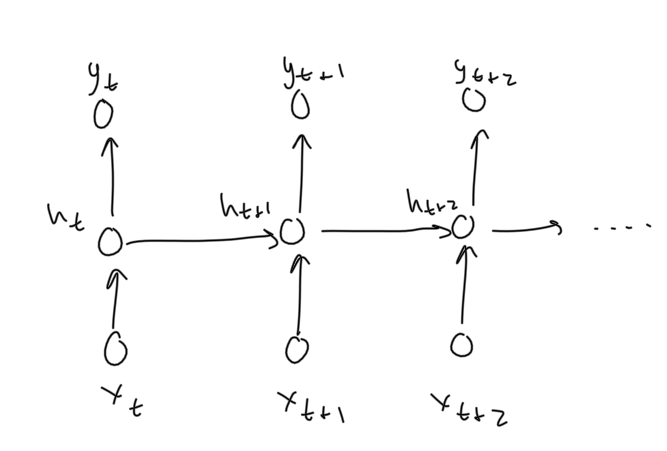
\includegraphics[width=0.5\paperwidth]{../NeuralNetworks/fig/RNN-structure.png}
    \caption{Simple example of an RNN.}
    \label{fig:RNN-structre}
\end{figure}


\subsection{Bayesian Neural Networks (BNNs)}
Up until now, our training process has been one of maximum likelihood estimation, or a maximum posterior approach if we utilize a regularizer that can be interpreted as introducing a prior.

A Bayesian neural network, or BNN, does exactly what you might imagine: it introduces a distribution over the parameters of our model, which then requires marginalizing over those distributions in order to make a prediction. The specifics of how exactly a BNN is constructed are beyond the scope of this textbook, but the idea behind why we would utilize a BNN is the same as the reason we utilize Bayesian techniques in other domains, particularly the use of prior information to aid model performance.
